\usepackage{amsthm}

\newtheorem{theorem}{Theorem}[chapter]
\newtheorem{lemma}           [theorem] {Lemma}   
\newtheorem{folg}           [theorem] {Folgerung}   

\newtheorem{frage}       [theorem] {Frage}   
\newtheorem{question}       [theorem] {Question}   
\newtheorem{aufgabe}       [theorem] {Aufgabe}   
\newtheorem{exercise}       [theorem] {Exercise}  

\newtheorem{proposition}     [theorem] {Proposition}  
\newtheorem{satz}     [theorem] {Satz}  
\newtheorem{fact}{Fact}
\newtheorem{definition}      [theorem] {Definition} 

\theoremstyle{definition} 
\newtheorem{bemerkung}     [theorem] {Bemerkung}  
\newtheorem{beispiel}       [theorem] {Beispiel}  
\newtheorem{example}       [theorem] {Example}  
\newtheorem*{example*} {Example}  
\newtheorem{notation}       [theorem] {Notation}  
\newtheorem*{Faust}[theorem]{Rule of Thumb}
\newtheorem*{Boxx}[theorem]{Concept}

The application of Taylor's formula is twofold: First, it gives a~polynomial that approximates a~given function quite fine in some neighbourhood. 
The second application is the computation of values of ``complicated functions''. We will present examples for both kinds of application.
\begin{example}
Consider the function $f(x)=\sin(x)$. We want to determine the Taylor polynomial of degree 6 with expansion point $x_0=\frac\pi2$. Since we have
$$
\sin'(x)=\cos(x),\quad\sin''(x)=-\sin(x),\quad\sin^{(3)}(x)=-\cos(x),
$$
$$
\sin^{(4)}(x)=\sin(x),\quad\sin^{(5)}(x)=\cos(x),\quad\sin^{(6)}(x)=-\sin(x)
$$
and
\[\sin(x_0)=\sin\left(\frac\pi2\right)=1,\quad \cos(x_0)=\cos\left(\frac\pi2\right)=0,\]
the Taylor polynomial of degree 6 is given by
\[T_6(x)=1-\frac12\left(x-\frac{\pi}{2}\right)^2+\frac{1}{24}\left(x-\frac{\pi}{2}\right)^4-\frac1{720}\left(x-\frac{\pi}{2}\right)^6.\]
The remainder term reads
\[R_6(x,x_0)=\frac{\sin^{(7)}(\hat{x})}{7!}\left(x-\frac{\pi}{2}\right)^{7}
=\frac{-\cos(\hat{x})}{5040}\left(x-\frac{\pi}{2}\right)^{7}.\]
    Taking into account that $|\cos(x)|\leq1$ for all $x\in\mathbb{R}$, we have that
\[|R_6(x,x_0)|\leq\frac{\left|x-\frac{\pi}{2}\right|^{7}}{5040}.\]
This leads to the estimate
\[|\sin(x)-T_6(x)|=|R_6(x,x_0)|\leq\frac{\left|x-\frac{\pi}{2}\right|^{7}}{5040}.\]

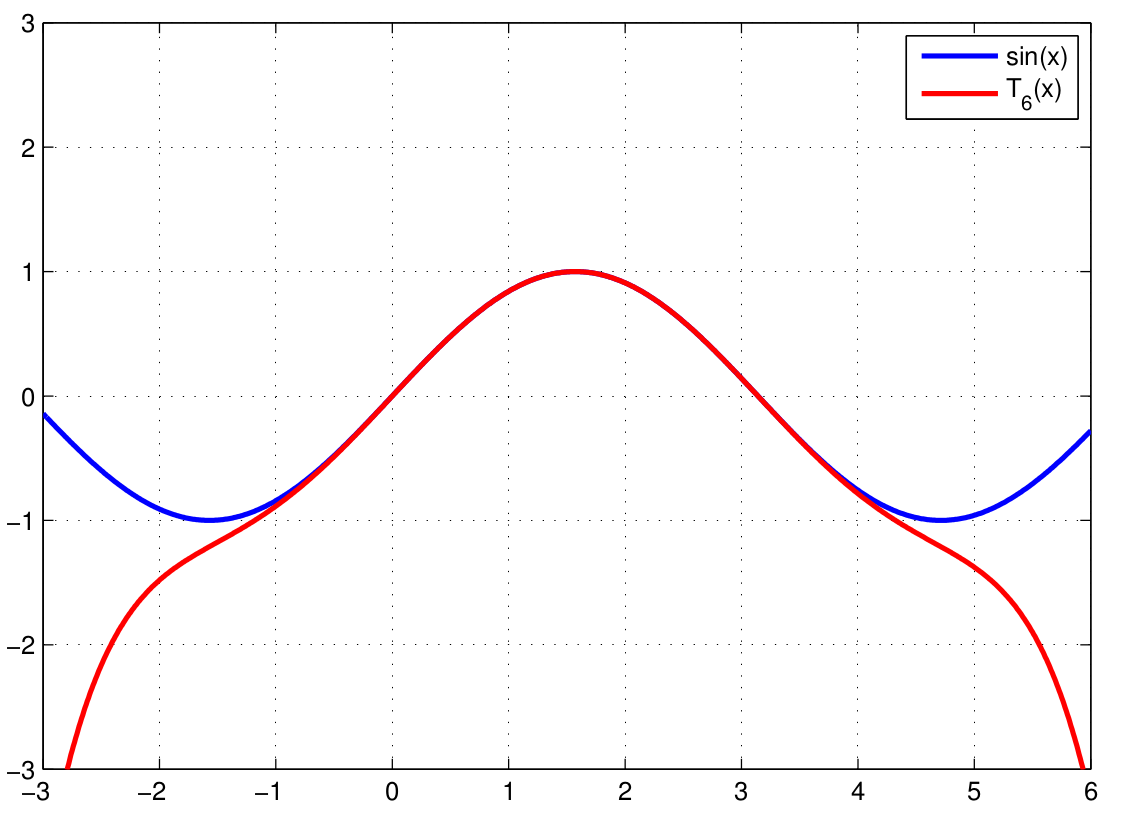
\includegraphics{./sin.png}

\end{example}
\begin{example}
We want to compute $\log(1.2)$ up to 3 digit precision. A~nice expansion point is $x_0=1$ since we know the precise values of $\log^{(k)}(1)$. Consider
$$
\log'(x)=\frac1x,\quad \log''(x)=-\frac{1!}{x^2},
$$
$$
\log^{(3)}(x)=\frac{2!}{x^3},\quad\log^{(4)}(x)=-\frac{3!}{x^4}
$$
and therefore, the Taylor polynomial of degree 3 is given by
\[T_3(x)=(x-1)-\frac12(x-1)^2+\frac13(x-1)^3.\]
In particular, we have
\[T_3(1.2)=0.2-\frac12\cdot 0.2^2+\frac13 \cdot 0.2^3=\frac{137}{750}.\]
Now we estimate $|\log(1.2)-\frac{137}{750}|$: The remainder term is given by
\[R_3(x,x_0)=-\frac{3!}{\hat{x}^4}\frac{(x-x_0)^{4}}{4!}=-\frac{(x-x_0)^{4}}{4\hat{x}^4}\]
for some $\hat{x}$ between $x$ and $x_0$. For $x=1.2$, $x_0=1$ we have $1<\hat{x}<1.2$ and therefore
\[ | R_3(1.2,1) | =\frac{(0.2)^{4}}{4\hat{x}^4}=4\cdot10^{-4}\frac{1}{\hat{x}^4}\leq4\cdot10^{-4}.\]
This leads to
\[|\log(1.2)-0.182\overline{6}|=|R_3(1.2,1)|\leq4\cdot10^{-4},\]
so we have determined $\log(1.2)$ up to three digits.
\end{example}

\begin{Theorem}\label{th:locext}
    Let $I\subset \mathbb{R}$ be an open interval, $n\in\mathbb{N}$ and $f:I\rightarrow\mathbb{R}$ an $n$-times continuously differentiable function. 
  Suppose that for $a\in I$ holds 
	$$f'(a)=f''(a)=\dots=f^{(n-1)}(a)=0\quad \text{and}\quad f^{(n)}(a)\neq 0 \ .$$
	If $n$ is odd, then $a$ is not a local extremum.
  If $n$ is even and $f^{(n)}(a)> 0$, then $a$ is a local minimum.
  If $n$ is even and $f^{(n)}(a)< 0$, then $a$ is a local maximum.   
\end{Theorem}

{\em Proof:} By assumption the Taylor expansion of $f$ of degree $n-1$ in the expansion point $a$ reads:
	\begin{equation}\label{eq:locext1} f(x)=f(a)+\frac{f^{n}(z)}{n!}(x-a)^n  \end{equation}
  where $z=z(x)$ lies between $x$ and $a$. Since $f^{(n)}$ is continuous and $f^{(n)}(a)\neq 0$,
  there is a neighbourhood $U:=~(a-\varepsilon,a+\varepsilon)~\subset I$, $\varepsilon>0$, of $a$ such that $f^{(n)}(x)\neq 0$ for all $x\in U$. 
  This means that for all $x\in U$, $f^{(n)}(x)$ and $f^{(n)}(a)$ have the same sign.
  Then for any $x_l \in~(a-\varepsilon,a)$ and any $x_r \in~(a,a+\varepsilon)$ Theorem \ref{th:locext} implies that for $z_l:=z(x_l)\in~(x_l,a)$ and $z_r:=z(x_r)\in~(a,x_r)$ holds
  $$
	  f(x_l) = f(a)+\frac{f^{n}(z_l)}{n!}(x_l-a)^n ,
  $$
  $$
	  f(x_r) = f(a)+\frac{f^{n}(z_r)}{n!}(x_r-a)^n
  $$
  and $0\neq f^{n}(a), f^{n}(z_l),f^{n}(z_r)$ have the same sign.
  If $n$ is odd,  then $(x_l-a)^n < 0 < (x_r-a)^n$  and therefore  either $f(x_l)<f(a)<f(x_r)$ or $f(x_l)>f(a)>f(x_r)$
  so that $a$ is not a local extremum.
  If $n$ is even and $f^{(n)}(a)>0$, then $(x_l-a)^n,(x_r-a)^n >0$ and $f(x_l),f(x_r)>f(a)$ so that $a$ is a local minimum.
  Finally, if $n$ is even and $f^{(n)}(a)<0$, then $(x_l-a)^n,(x_r-a)^n >0$ and $f(x_l),f(x_r)<f(a)$ so that $a$ is a local maximum.
$\Box$

